% Format teze zasnovan je na paketu memoir
% http://tug.ctan.org/macros/latex/contrib/memoir/memman.pdf ili
% http://texdoc.net/texmf-dist/doc/latex/memoir/memman.pdf
% 
% Prilikom zadavanja klase memoir, navedenim opcijama se podešava 
% veličina slova (12pt) i jednostrano štampanje (oneside).
% Ove parametre možete menjati samo ako pravite nezvanične verzije
% mastera za privatnu upotrebu (na primer, u b5 varijanti ima smisla 
% smanjiti 
\documentclass[12pt,oneside]{memoir}
% Paket koji definiše sve specifičnosti mastera Matematičkog fakulteta
\usepackage{matfmaster}
%
% Podrazumevano pismo je ćirilica.
%   Ako koristite pdflatex, a ne xetex, sav latinički tekst na srpskom jeziku
%   treba biti okružen sa \lat{...} ili \begin{latinica}...\end{latinica}.
%
%
% Opicija [latinica]:
%   ako želite da pišete latiniciom, dodajte opciju "latinica" tj.
%   prethodni paket uključite pomoću: \usepackage[latinica]{matfmaster}.
%   Ako koristite pdflatex, a ne xetex, sav ćirilički tekst treba biti
%   okružen sa \cir{...} ili \begin{cirilica}...\end{cirilica}.
%
% Opcija [biblatex]:
%   ako želite da koristite reference na više jezika i umesto paketa
%   bibtex da koristite BibLaTeX/Biber, dodajte opciju "biblatex" tj.
%   prethodni paket uključite pomoću: \usepackage[biblatex]{matfmaster}
%
% Opcija [b5paper]:
%   ako želite da napravite verziju teze u manjem (b5) formatu, navedite
%   opciju "b5paper", tj. prethodni paket uključite pomoću: 
%   \usepackage[b5paper]{matfmaster}. Tada ima smisla razmisliti o promeni
%   veličine slova (izmenom opcije 12pt na 11pt u \documentclass{memoir}).
%
% Naravno, opcije je moguće kombinovati.
% Npr. \usepackage[b5paper,biblatex]{matfmaster}

% Pomoćni paket koji generiše nasumičan tekst u kojem se javljaju sva slova
% azbuke (nema potrebe koristiti ovo u pravim disertacijama)
% Datoteka sa literaturom u BibTex tj. BibLaTeX/Biber formatu
\usepackage{multirow}
\usepackage{dcolumn}
\usepackage{amsthm}
\usepackage{tabularx}
\usepackage{ltablex} 
\usepackage{lscape}
\usepackage{booktabs}
\usepackage{enumitem}
\usepackage{listings}
\usepackage{amsmath,amssymb,latexsym}
\usepackage[unicode]{hyperref}
\usepackage{subfig}
\hypersetup{colorlinks,citecolor=green,filecolor=green,linkcolor=blue,urlcolor=blue}
\renewcommand{\lstlistingname}{Код}
 
\newtheorem{definic}{Дефиниција}
\bib{master_branislavaz}

% Ime kandidata na srpskom jeziku (u odabranom pismu)
\autor{Бранислава Б. Живковић}
% Naslov teze na srpskom jeziku (u odabranom pismu)
\naslov{Паралелизација статичке верификације софтвера }
% Godina u kojoj je teza predana komisiji
\godina{2017}
% Ime i afilijacija mentora (u odabranom pismu)
\mentor{др Милена Вујошевић Јаничић, доцент\\ Универзитет у Београду, Математички факултет}
% Ime i afilijacija prvog člana komisije (u odabranom pismu)
\komisijaA{др Саша Малков, ванредни професор\\ Универзитет у Београду, Математички факултет}
% Ime i afilijacija drugog člana komisije (u odabranom pismu)
\komisijaB{др Филип Марић, ванредни професор\\ Универзитет у Београду, Математички факултет}
% Ime i afilijacija trećeg člana komisije (opciono)
% \komisijaC{}
% Ime i afilijacija četvrtog člana komisije (opciono)
% \komisijaD{}
% Datum odbrane (obrisati ili iskomentarisati narednu liniju ako datum odbrane nije poznat)
\datumodbrane{ 2017.}

% Apstrakt na srpskom jeziku (u odabranom pismu)
\apstr{%
}

% Ključne reči na srpskom jeziku (u odabranom pismu)
\kljucnereci{паралелизација, верификација, рачунарство}

\begin{document}
% ==============================================================================
% Uvodni deo teze
\frontmatter
% ==============================================================================
% Naslovna strana
\naslovna
% Strana sa podacima o mentoru i članovima komisije
\komisija
% Strana sa posvetom (u odabranom pismu)
%\posveta{Брату, мами и тати}
% Strana sa podacima o disertaciji na srpskom jeziku
%\apstrakt
\mainmatter
% Sadržaj teze
\tableofcontents

% ==============================================================================
% Glavni deo teze
% ==============================================================================

% ------------------------------------------------------------------------------
%\chapter{Увод}
% ------------------------------------------------------------------------------



\chapter{Увод} 

 Развој и примена нових технологија почињу све више да утичу на друштво. Рачунари су присутни свуда око нас и пружају нам многе погодности и олакшице како у необавезним тако и у пословним активностима. Институције попут банака, здравства, просвете, и других теже да аутоматизују своје процесе коришћењем разних софтверских алата.  
 
 Грешке у софтверу могу имати катастрофалне последице, на пример отказивање медицинског уређаја у току операције или отказивање аутоматског пилота у току лета. Како бисмо предухитрили овакве ситуације, потребно је детаљно и прецизно утврдити исправност развијеног софтвера. 
 
  Испитивање исправности софтвера може бити динамичко и статичко. Статичка верификација софтвера представља најпоузданији начин испитивања исправности програма, уз битна теоријска ограничења, јер се многи аспекти коректности програма не могу алгоритамски испитати ( нпр. неодлучивост Халтинг проблема \cite{halting} нам говори да није могуће направити алгоритам којим би се испитало да ли се произвољни дати програм зауставља). 
  
\subsection{Мотивација}

 Аутоматизовано статичко утврђивање исправности софтвера захтева анализу програмског кода без његовог извшавања, коришћењем техника статичке анализе. Ове технике могу бити веома сложене и могу захтевати доста времена и ресурса, што додатно ограничава сам процес.

 Алати за аутоматску статичку верификацију софтвера због свих поменутих ограничења могу бити веома комплексни, због чега је погодно покретати их на рачунарима са јаким хардверским перформансама. Временом су процесори са више језгара почели да доминирају тржиштем и данас готово сваки нов рачунар садржи вишејезгарни процесор. Такође, рачунари са више процесора постају све доступнији. Због тога софтвер који имплементира конкурентно ивршавање и користи сав потенцијал вишепроцесорских и вишејезгарних система добија на значају.
 
 У оквиру овог рада надограђен је систем за аутоматску верификацију софтвера \textit{LAV} \cite{mvjphd}. Процес испитивања исправности програма је паралелизован на два нивоа (испитивање исправности блокова наредби и испитивање исправности функција) и приказани су експериментални резултати поређења секвенцијалног и паралелног извршавања система \textit{LAV} као и експериментално поређење са алатом \textit{CBMC} \cite{cbmc}. Резултати показују да паралелизација може значајно да убрза процес утврђивања исправности програма.

%Испитивање задовољивости логичке формуле је НП-комплетан проблем и један је од најтежих проблема у рачунарству.


\chapter{Верификација софтвера}
	Верификација софтвера представља дисциплину рачунарства која се бави провером и доказивањем исправности програма. Програм је исправан уколико задовољава задату спецификацију, односно уколико за сваки улаз има одговарајуће понашање које је предвиђено спецификацијом. Постоје два основна приступа верификацији, \textit{динамичка} и \textit{статичка} верификација.
  
  
  \section{Статичка верификација}
  \label{statver}
  Статичка верификација програма представља испитивање исправности програма анализом програмског кода, без његовог извршавања. Анализа програмског кода се врши углавном над изворним или објектним кодом. Особине програма и услови исправности се описују одговарајућим формулама изабране математичке теорије. Изграђене формуле се даље анализирају коришћењем стриктних математичких метода. Многа питања релевантна за верификацију су неодлучива (на пример, питање да ли се програм зауставља или да ли је нека наредба у програму достижна) и стога није могуће утврдити да ли је програм потпуно исправан. Због тога се особине програма апроксимирају и описују одлучивим математичким теоријама. Аутоматизоване технике статичке анализе су \textit{проверавање модела}, \textit{апстрактна интерпретација} и \textit{симболичко извршавање}.  
  
\paragraph{Проверавање модела} је техника верификације која на основу датог програма конструише одговарајући модел и испитује да ли он задовољава одговарајућу спецификацију. Програм се описује коначним аутоматом који се састоји од стања и прелаза између стања, а спецификација се описује формулом темпоралне логике. Испитивање исправности програма се врши систематским обиласком свих могућих стања аутомата како би се доказали услови задати спецификацијом. Уколико доказивање није могуће, генерише се одговарајући контрапример. Овај процес може бити веома дуг и исцрпан уколико је број могућих стања аутомата велики. Основни проблем ове технике је комбинаторна експлозија до које може доћи уколико повећавамо број променљивих у програму. Са повећањем броја променљивих скуп могућих стања аутомата ће експоненцијално порасти што додатно продужује време потребно за њихов обилазак \cite{mvjphd,verif_tech}.

\paragraph{Апстрактна интерпретација} представља методу верификације код коje се семантика програма апроксимира математичким моделом. Модел понашања програма се описује конкретним доменом и одговарајућим релацијама над њиме. Анализа оваквог модела је отежана у случајевима када је конкретан домен јако велики, због чега се конкретан домен апроксимира апстрактним доменом. На пример, домен скупа целих бројева се може заменити скупом који садржи знакове бројева $ \{+,-,0\}$. Анализом апстрактног домена може се испитати важење неких својстава програма без његовог извршавања. Међутим, апстраховање домена такође може довести до губитка неких информација што смањује прецизност ове методе и често повећава број лажних упозорења, али повећава скалабилност ове технике. Апстрактна интерпретација се такође може применити и у оквиру трансформације или оптимизације програма као и приликом аутоматског одређивања инваријанти петљи \cite{mvjphd,verif_tech}. 

\paragraph{Симболичко извршавање} је метода верификације која анализира понашање програма на основу конструисаних симболичких израза. Конкретне вредности променљивих се замењују симболичким вредностима, а изабране путање програма се описују симболичким изразима. Испитивање исправности програма се врши анализом конструисаних израза и уколико се за неку путању закључи да је исправна, онда тај закључак важи за све могуће улазе који прате ту путању. Ова метода је прецизна метода али често недовољно ефикасна. Број могућих путања кроз програм може да буде јако велики што отежава њихову анализу. Због тога се ова метода углавном користи приликом проналажења грешака у програму а не за комплетну верификацију \cite{mvjphd,symbolic_exec}.

\section{Динамичка верификација}
  Динамичка верификација програма се врши током његовог извршавања. Грешке у програму се покушавају пронаћи исцрпним тестирањем. Битно је нагласити да тестирањем није могуће доказати исправност програма већ је у неким случајевима могуће пронаћи неке грешке и на тај начин оповргнути претпоставку о исправности програма. 
  
   Да би се програм тестирао потребно је пронаћи одговарајући скуп улазних података помоћу којих се врши тестирање.  С обзиром на то да је простор могућих улаза углавном превелики, није могуће тестирати програм за све могуће улазе. Због тога треба издвојити одговарајући подскуп улазних података који што боље описује спецификацију програма и покривају што већи број случајева. Избор улазних података се углавном врши на основу анализе програмског кода и спецификације. 
   
    Постоје две основне методе динамичког тестирања, метода \textit{црне} и 
 \textit{беле} кутије.  Методом црне кутије генерисање тестова се врши на основу спецификације програма не узимајући у обзир детаље имплементације. Методом беле кутије тестови се генеришу на основу кода и структуре програма. Такође, постоји и метода сиве кутије који представља мешавину ова два приступа. У зависности од тога шта је потребно тестирати користи се одговарајућа метода \cite{testing}. 
  
  \section{Међујезици у верификацији}
  
  Програми писани на вишим програмским језицима су често веома сложени и анализа њиховог изворног кода може бити веома компликована. Присуство сложених наредби, разних конверзија и бочних ефеката додатно отежава анализу изворног кода. Због тога се често, програм писан на вишем програмском језику, трансформише у међујезик који је погодан за анализу. Постоје разне платформе које трансформишу програм у облик погодан за анализу, неке од њих су \textit{LLVM} и \textit{.NET} платформа. У наставку ће бити описана \textit{LLVM} платформа јер је она коришћена приликом имплементације.
  
  \paragraph{LLVM} \cite{llvm} пројекат је започет на Универзитету Илиноис са циљем да пружи подршку за компилацију различитих програмских језика. Пројекат је отвореног кода и има широку примену у индустрији и науци. Временом се пројекат проширио и данас се састоји од различитих потпројеката који се користе у производњи и верификацији софтвера. Основни потпројкат садржи алате и библиотеке за трансформацију, анализу и оптимизацију програма независно од изворног кода. Међујезик који користе ови алати се зове \textit{LLVM} међујезик у који је могуће превести бројне више програмске језике попут \textit{C}, \textit{C++}, \textit{Java}, \textit{Python} и друге.
  
  \section{Алати за верификацију}
У наставку ће бити описани неки верификациони алати који користе поменуте технике приликом испитивања исправности програма. Ови алати могу да пронађу грешке као што су дељење нулом, прекорачење бафера, неисправно и двоструко ослобађање меморије, прекорачење у аритметичким изразима и друге. Такође, могу да проверавају и неке додатке услове које задаје корисник.

\paragraph{LLBMC (енг. Low-Level Bounded Model Checker)} је алат који проверава исправност 
\textit{C} и \textit{C++} програма. Користи технике за проверавање ограничених модела над \textit{LLVM} међукодом. За проверавање услова исправности користи \textit{SMT} решаваче \textit{STP} i \textit{Boolector} \cite{llbmc}.

\paragraph{KLEE} је алат који врши симболичко извршавање и генерисање тест примера над програмима који су писани на језику \textit{C}. Настао је на Универзитету Илиноис и јавно је доступан. \emph{KLEE} анализира \emph{LLVM} међукод користећи \textit{SMT} решавач \textit{STP} приликом испитивања услова исправности \cite{klee}. 

\paragraph{CBMC} је алат за верификацију \textit{C} и \textit{C++} програма првенствено намењен за верификацију уграђених система (енг. \textit{embedded systems}). \textit{CBMC} врши симболичко израчунавање тако што изворни код програма преводи у \textit{SAT} формулу и испитује њену задовољивост \cite{cbmc}. 

\section{Систем LAV}
	\textit{LAV} је алат за статичку верификацију софтвера \cite{mvjphd}. Oтвореног је кода и јавно је доступан \cite{lav_online}. 
	
	\textit{LAV} имплементира статичку анализу, генерисање и испитивање услова исправности императивних програма комбинујући методе описане у поглављу \ref{statver}. Користи \textit{LLVM} инфраструктуру ради трансформисања програма у облик који је погодан за анализу и првенствено је намењен за анализу програма написаних у програмском језику \textit{C}. Међутим, универзалност платформе \textit{LLVM} омогућава и анализу других процедуралних језика који се могу компилирати у \textit{LLVM} код, као што су језици \textit{C++}, \textit{Ada} и \textit{Fortran}. \textit{LAV} моделује понашање програма и генерише услове исправности трансформишући их у формуле одговарајуће теорије логике првог реда. Теорије које су подржане су аритметика бит-вектора, линеарна аритметика, теорија неинтерпретираних функција (или акерменизација) и теорија низова \cite{smt}.  Симболичким извршавањем \textit{LAV} генерише формуле изабране теорије логике првог реда које описују понашање сваког блока \textit{LLVM} међукода као и њихове релације. 
	
	\textit{LAV} генерише формуле услова исправности неке наредбе и испитује њихову задовољивост користећи \textit{SMT} решавач. Комбинацијом ових формула граде се формуле које описују понашање програма. 
	
	 Формуле се конструишу по потреби у различитим контекстима. Контекст обухвата информације из околине наредбе које ће бити узете у разматрање приликом расуђивања о наредби. Разматрају се празан контекст, контекст блока, контекст функције и контекст у коме је функција позвана. Наведени су према ширини од најужег до најширег. Приликом испитивања исправности наредбе почиње се од празног контекста.  Након генерисања формуле у оквиру једног контекста, формула се шаље \textit{SMT} решавачу на проверу. У зависности од резултата испитивање се наставља у ширим контекстима. 
	 
 На основу резултата решавача, \textit{LAV} генерише извештај о исправности наредби програма \cite{mvjdev}. 	
	 
	
\chapter{Основе паралелизације}
	Термини паралелизам и конкурентност у рачунарству су углавном испреплетани и погрешно схваћени. Често се грешком поистовећују и сматрају синонимима иако то нису. Због тога је битно да их правилно дефинишемо и разликујемо \cite{par_computing}.
%\begin{definic}
%	Конкурентност је својство програма које се односи на то да два или више задатака могу бити истовремено у току. (исправити превод)
%\end{definic}
%\begin{definic}
%	Паралелизам је својство програма да извршава два или више задатака истовремено. (исправити превод)
%\end{definic}

\begin{definic}
	За два процеса кажемо да се извршавају конкурентно ако није унапред позната њихова међусобна временска лоцираност.
\end{definic}
\begin{definic}
	Два процеса се извршавају паралелно ако постоји период времена у коме су оба процеса истовремено активни
\end{definic}

Битно је напоменути да постоји разлика у томе да ли се два задатка истовремено извршавају или су истовремено у току. Конкурентни програми се могу извршавати паралелно али не морају. Паралелизам захтева архитектуру која има више процесорских јединица, док се конкурентност може остварити и на једном процесору.

 	Паралелно програмирање је област рачунарства која се бави архитектуром система и софтверским проблемима програма са паралелним извршавањем. Програм се може дефинисати као низ наредби које се извршавају након његовог покретања. Секвенцијалне програме одликује серијско извршавање наредби. Паралелизам је карактеристика програма која се односи на несеквенционалност његових израчунавања. Независна израчунавања се могу истовремено односно паралелно извршавати на више процесорских јединица.
 	
 	Инстанца програма која се извршава на једном процесору назива се \textit{процес}. Текуће стање процеса обухвата информације о извршавању и управљању ресурсима. Прелазак са извршавања једног процеса на процесору на извршавање другог процеса назива се промена контекста. Промена контекста захтева замену стања првог процеса стањем другог процеса и може одузети значајно време, због чега процеси могу бити веома скупи. Процеси не деле ресурсе међу собом и њихова комуникација се врши коришћењем посебних механизама, што додатно подиже цену коришћења процеса. Цена коришћења процеса се може смањити увођењем \textit{нити}. Нит представља компоненту процеса која се извршава секвенцијално. Процес може имати више нити и оне међусобно деле ресурсе помоћу којих могу комуницирати \cite{apue}. 
 	
 	  
 	
  \section{Мотивација}
  Интересовање за паралелизацију се јавља касних 1950-их, са зачетком теоријских основа, док се први технички напредак осећа почетком 1960-их и и даље расте. Први суперрачунари су се појавили 60-их година и имали су више процесора који су могли паралелно да раде са дељеном меморијом. Даљим развојем 80-их година се појављују кластери, системи који се састоје од великог броја рачунара, тзв. чворова, међусобно повезаних преко мреже. 90-их година са експанзијом интернета се појављује рачунарство у облаку, док данас већина кућних рачунара садржи процесоре са више језгара. 
  
   Може се рећи да перформансе рачунара експоненцијално расту од 1945 године за фактор 10 сваких 5 година. Први рачунари су израчунавали десетине операција са бројевима у покретном зарезу у секунди, паралелни рачунари 1990-их достижу број од више десетина милијарди операција у секунди \cite{par_history}.
   
    Перформансе софтверских решења зависе од времена извршавања основних операција, попут операција са бројевима у покретном зарезу, као и од броја оваквих операција које се могу извршавати паралелно. С обзиром на то да ово време зависи од брзине откуцаја часовника процесора, која полако тежи ка теоријском максимуму (који је последица брзине кретања сигнала кроз проводнике и дужине проводника), не можемо се ослонити на то да ће и у даљој будућности повећавање брзине откуцаја часовника моћи да значајно подигне перформансе нумеричких израчунавања.
    Поред тога, Муров закон \cite{moore} нам говори да ће се на сваких осамнаест месеци број транзистора на једном процесорском језгру дуплирати. С обзиром на то да постоји теоријско ограничење величине транзистора, тј. величина атома, овај експоненцијални раст није одржив. Због тога се напредак у овом смеру покушава остварити на другачији начин, повећањем броја процесорских језгара. Захваљујући овоме убрзање програма  се може постићи коришћењем разних техника паралелизације.
    
     \textit{Фактор убрзања паралелизацијом} је број који показује колико пута се програм извршаван на више процесора извршава брже него када се тај исти програм извршава на једном. Формула убрзања је следећа \cite{par_various}:
 	$$ S = T_s/T_p $$
 	
\noindent где $ T_s $ представља време извршавања програма на једном процесору а $ T_p $ време извршавања програма на више процесора. 

 По Амдаловом закону \cite{par_various}, извршавање паралелног програма на паралелном рачунару углавном обухвата и део операција које се не могу извршавати паралелно. Означимо са $ \alpha $ део програма који се мора извршавати секвенцијално на једном процесору, а остатак $ (1 - \alpha)$ се може извршити паралелно. Ако је $ N $ број процесорских јединица, формула убрзања је: 
 	$$ S = 1 / ( \alpha + (1-\alpha)/N)$$
Ова формула нам показује да убрзање никада не може прећи $ 1/\alpha $, тј. број процесорских јединица не утиче на део програма који се мора извршавати секвенцијално. На слици \ref{fig:amdal} је приказана зависност убрзања од броја процесора и дела посла који се мора обавити секвенцијално. Битно је нагласити да конкурентан програм на једном процесору може да буде неефикаснији од секвенцијалног.

 \begin{figure}[!ht]
  \centering
  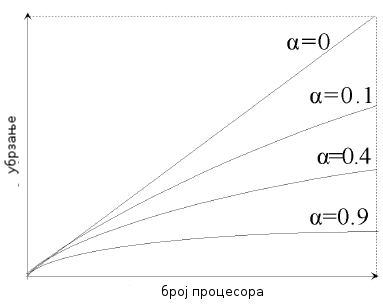
\includegraphics[width=0.8\textwidth]{img/amdal.png}
  \caption{Зависност убрзања од броја процесора}
  \label{fig:amdal}
\end{figure}



 У пракси, време извршавања програма на паралелним системима је углавном мање од теоријски израчунате вредности, а само у неким случајевима је веће. Амдалов модел разматра само случајеве у којима је димензија проблема фиксирана и постоји тачно једно уско грло (углавном процесор). Најчешће постоји више уских грла, што има већи утицај него други фактори. Поред Амдаловог модела постоје и други модели као што су Густафсонов, Гинтеров, модел Сун Ни-ја који превазилазе нека ограничења Амдаловог модела \cite{performance}.


  \section{Врсте паралелизације}
  
 Програми се могу паралелизовати на различите начине. Паралелизацију може обављати програмер експлицитно или коришћењем неких алата. Последњих година развијене су многе алатке који омогућују аутоматску паралелизацију. Коришћењем ових алатки програмеру је олакшан процес паралелизације уз ограничену контролу. Овакав начин паралелизације је погодан за велике и комплексне системе код којих би ручна паралелизација била спора и компликована.
 
  Са друге стране, ручна паралелизација програма захтева добро обучене програмере и углавном је сложенија али пружа програмерима потпуну контролу над самим процесом паралелизације. Овакав приступ је погоднији за паралелизацију специфичних проблема.


  Битно је нагласити да није могуће паралелизовати све делове сваког алгоритма. Посао програмера је да пронађе и одлучи који делови алгоритма се могу паралелизовати и на који начин.
 Два најчешћа приступа дизајнирању паралелних алгоритама су \textit{паралелизација задатака} и \textit{паралелизација података} \cite{art_conc}. 
Паралелизација задатака представља дељење алгоритма на независне задатке који се могу извршавати било којим редоследом над истим скупом података.
Паралелизација података представља дељење података тако да се један задатак може независно извршавати над дисјунктним деловима података било којим редоследом \cite{art_conc}. 
На слици  \ref{fig:data_parallel} је приказан пример паралелизације задатака а на слици \ref{fig:task_parallel} пример паралелизације података

\begin{figure}[!ht]
  \centering
  \includegraphics[width=0.6\textwidth]{img/data_parallel.png}
  \caption{Пример паралелизације података: примена функције \textit{toupper} над сваким словом појединачно}
  \label{fig:data_parallel}
\end{figure}

\begin{figure}[!ht]
  \centering
  \includegraphics[width=0.6\textwidth]{img/task_parallel.png}
  \caption{Пример паралелизације задатака: примена различитих функција над истим подацима}
  \label{fig:task_parallel}
\end{figure}


  \section{Изазови процеса паралелизације}
  Често није могуће поделити алгоритам на потпуно независне задатке који се могу паралелно извршавати већ је присутан одређен ниво зависности између њих. На пример, уколико задаци могу приступити истој променљивој у програму и променити њену вредност, потенцијално више задатака може истовремено покушати да је измени. У таквим ситуацијама задаци се надмећу за приступ дењеним подацима.  Овакви и овоме слични проблеми индукују постојање \textit{синхронизације}. Због тога постоје бројна решења и механизми који омогућавају \textit{комуникацију} и  \textit{синхронизацију} између задатака.
  
  
Комуникација представља било који вид размене информација између задатака. Може се остварити преко дељене меморије или слањем односно примањем порука. Комуникација преко порука се одвија тако што један задатак експлицитно шаље другом задатку податке да их прихвата и обрађује. Неки од познатих механизама за овакав вид комуникације су сигнали, цеви, сокети и канали.
Постојање дељене меморије има своје добре и лоше стране. Понекад је потребно старати се о редоследу читања односно писања дељене меморије као и о евентуалним утркивањима и сукобима. Због тога комуникација преко дељене меморије може захтевати додатну синхронизацију. Помоћу механизама синхронизације програмер може контролисати редослед извршавања задатака и приступања дељеној меморији. Две основне врсте овакве синхронизације су \textit{сарадња} и \textit{такмичење}. Синхронизација сарадње између два задатка је потребна уколико један задатак зависи од резултата рада другог. Синхронизација такмичења је неоходна у случајевима када два задатка истовремено захтевају исти ресурс. Механизми који се користе за имплементацију синхронизације су мутекси, катанци, семафори, монитори и други \cite{lang_prag}.

 Синхронизација отвара многе проблеме, нпр. могућност \textit{узајамног блокирања} и \textit{изгладњивања} између задатака. Ови проблеми се односе на концепт \textit{напредовања} (енг. \textit{liveness}) програма. Концепт напредовања програма представља својство програма да у току свог извршавања напредује према очекиваном резултату рада , односно да константно прави прогрес током свог извршавања. Уколико ово својство није задовољено може да се деси да програм не може да настави са својим извршавањем. Узајамно блокирање (енг. \textit{deadlock}) се дешава у ситуацији када два задатка чекају један на другог како би наставили са радом и због тога не остварују напредак. Живо блокирање (енг. \textit{livelock}) представља ситуацију када неки од блокираних задатака раде али нема напретка. Изгладњивање се односи на могућност да један задатак спречава извршавање другог учесталим резервисањем заједничког ресурса. Поменути проблеми се могу спречити одговарајућим алгоритмима \cite{opsis}.


 % \section{Неки патерни}
  \section{Библиотеке за паралелизацију}
	У овом поглављу ће бити описане неке библиотеке које се користе за паралелизацију програмског кода. Акценат ће бити на библиотекама за језик \textit{C++}. 
	
 Алатке за паралелизацију можемо поделити у две категорије: \textit{имплицитне} и \textit{експлицитне}. Имплицитне алатке олакшавају програмеру имплементацију паралелних алгоритама јер се старају о прављењу, управљању и синхронизацији нити. Експлицитни алати пружају већу флексибилност и контролу захтевајући од програмера да управља свим аспектима вишенитности.
\paragraph{Подршка за паралелизацију у оквиру стандардне библиотеке језика \textit{C++}}

Стандардна библиотека нуди уграђену подршку за управљање нитима, закључавањем колекција, атомичним подацима и асинхроним позивањем и чекањем резултата. Нека од заглавља у којима су имплементиране потребне структуре и фунцкије су:
\begin{description}
	\item[\texttt{<thread>}] - Дефинише класу \texttt{thread} која служи за конструкцију и управљање нитима. Конструктор ове класе може прихватити функцију коју ће нит извршавати. Овако конструисана инстанца има свој јединствени идентификатор и налази се у стању извршавања (\textit{joinable}). Позивом функције \texttt{join()} над објектом нити можемо сачекати да нит заврши са извршавањем односно позивом функције \texttt{detach()} можемо откачити нит и дозволити да настави своје извршавање независно од главне нити. Још неке од корисних функција су: \texttt{hardware\_concurrency()} - враћа број нити које су подржане на систему \footnote{Овај број не мора нужно бити број физичких језгара на систему.}, \texttt{native\_handle()} - враћа објекат помоћу кога се управља датом нити и друге.
	\item[\texttt{<atomic>}] - Садржи компоненте које обезбеђују атомичне податке, т.ј. податке који су безбедни приликом рада у конкурентном окружењу. Класа \texttt{atomic} представља атомичан податак са јасно дефинисаним понашањем у ситуацијама када две или више нити покушају да раде са њиме. Шаблон ове класе је применљив на било који тип. Неке од корисних функција су: \texttt{load()} - враћа вредност податка, \texttt{store(druga\_vrednost)} - замењује тренутни податак другим податком, \texttt{fetch\_add(druga\_vrednost)} - додаје вредност на тренутнy вредност и друге.
	\item[\texttt{<future>}] - Олакшава асинхронo извршавање задатака као и приступ и управљање вредностима које су направљене асинхроно. Функција \texttt{async} асинхроно извршава функцију која јој је прослеђена као аргумент и њен резултат смешта у објекат типа \texttt{future}. Објекат типа \texttt{future} омогућава чекање на резултат док се асинхрона функција не заврши. Уколико је потребно да више нити чека на резултат асинхроног извршавања функције, резултат је потребно сместити у објекат типа \texttt{shared\_future} чије коришћење је безбедно у вишенитном контексту. Чекање на међурезултате чије вредности се могу поставити у другим нитима се може постићи коришћењем објекта типа \texttt{promise}.    
%	\item[\texttt{<functional>}] - Пружа подршку за рад са објектима који су посебно дизајнирани тако да се могу користити као функције. Такви објекти се називају функционални објекти. Инстанце класе \texttt{std::function} представљају један пример таквих објеката. Функција \texttt{bind(fun\_objekat, arg1, arg2, ...)}  везује један или више аргумента функционалног објекта, другим речима врши парцијалну апликацију функције на прослеђене аргументе.   
\end{description}

\paragraph{ PThreads (енг. POSIX Threading interface) \cite{pthread}}је интерфејс за паралелно програмирање на нивоу оперативног система и доступан је у оквиру већине \textit{UNIX}-оликих оперативних система. Имплементиран је у оквиру библиотеке \texttt{pthread.h} језика \textit{C} који садржи скуп константи, типова и функција за паралелизацију. Програмеру је омогућено прављење нити и управљање њиховим извршавањем. Комуникација се обавља преко дељене меморије коју такође програмер контролише. Дељена меморија се имплементира коришћењем глобалних променљивих које су видљиве свим нитима. 

\paragraph{OpenMP (енг. Open Specification for Multi-Processing) \cite{openmp}} је интерфејс за програмирање који омогућава паралелно програмирање у језицима \textit{C}, \textit{C++} и \textit{Fortran} . Заснива се на моделу паралелизације коришћењем дељене меморије. Садржи скуп компаjлерских директива, рутина и глобалних променљивих које служе за обележавање делова програмског кода. Програм се дели на регионе који се извршавају серијски и регионе који се извршавају паралелно. Региони се означавају директивама које управљају процесом додељивања задатака нитима, комуникацијом и синхронизацијом. Променљиве могу бити дељене, односно видљиве свим нитима, и приватне, односно видљиве у оквиру нити унутар које су декларисане.

\paragraph{TBB (енг. Thread Building Blocks) \cite{tbb}} је \textit{C++} библиотека за паралелно програмирање на вишепроцесорским системима развијена од стране \textit{Intel}-а. Библиотека се састоји од бројних шаблона који имплементирају паралелне алгоритме, контејнере, примитиве за синхронизацију и управљач задацима. Програмери дефинишу задатке који ће се извршавати паралелно након чега се управљач задацима стара о току извршавања и техничким детаљима.
  
\chapter{Модул за паралелизацију}

Mодул који се бави паралелизацијом је развијен у складу са специфичним захтевима система \textit{LAV}. Систем \textit{LAV} је сложен верификациони алат писан на језику \textit{C++}. Користи многе спољне библиотеке, алатке, као и \textit{SMT} решаваче.  Архитектура самог система је модуларна, функционалне целине су издвојене у посебне модуле и по потреби увезиване и коришћене. Модул за паралелизацију представља посебну издвојену целину тако да се може користити у различитим деловима система. Имплементиран је коришћењем библиотека језика \textit{C++}. У наставку текста ће бити описана архитекура и имплементација модула за паралелизацију као и начини његовог коришћења у оквиру система \textit{LAV}. Изворни код модула је јавно доступан \footnote{Може се пронаћи на адреси \url{http://argo.matf.bg.ac.rs/?content=lav} (директоријуми \texttt{include/lav/Threads} и \texttt{lib/Threads}) а интеграција са \textit{LAV}-ом се налази унутар класа \texttt{LBlock}, \texttt{LModule} и \texttt{LState}.}.  

\section{Опис проблема}
Процес верификације у систему \textit{LAV} је имплементиран секвенцијално. На улазу се задаје модул (скуп датотека) који је потребно анализирати.  \textit{LAV} разлаже модул на његове функције и почев од \texttt{main} функције (уколико се почетна функција не зове \texttt{main} њено име се може задати приликом покретања система \textit{LAV}) прави граф позива функција  на основу кога се функције верификују. Даље, функције се разлажу на блокове, а блокови на појединачне наредбе. Симболичким извршавањем конструише се \textit{SMT} формула која описује услов исправности неке потенцијално небезбедне наредбе. \textit{SMT} решавачу се на проверу шаље негација ове формуле и уколико је она незадовољива, онда то значи да је употреба одговарајуће наредбе исправна. Уколико се за потенцијално неисправне наредбе једног блока покаже да су исправне, онда то значи да је анализирани блок исправан. Уколико су сви блокови унутар једне функције исправни, онда је и сама функција исправна. Слично важи и за модул. 

Као што знамо, програми могу бити комплексни, са великим бројем функцијa (блокова и наредби), због чега и овај процес може бити дуг. Додатно, функције често позивају једна другу што значи да могу бити међусобно зависне. Због тога, неретко се догађа да функција \textit{A} позива функцију \textit{B}, функција \textit{B} позива функцију \textit{C}, док је функција \textit{D} неисправна али њена верификација се секвенцијалним приступом може обавити тек након што се заврши верификација функција \textit{A}, \textit{B} и \textit{C}. Ова и сличне ситуације су биле мотивација за паралелизацију процеса верификације. 

Паралелизација је имплементирана на два нивоа. Први ниво је паралелно верификовање различитих наредби у оквиру једног блока, а други ниво је паралелно верификовање самих функција.

Систем \textit{LAV} имплементира алгоритам који услове исправности програма описује формулама изабране логике првог реда и испитује њихову задовољивост.  Испитивање задовољивости је  временски веома захтевно и може да варира у зависности од формуле. \textit{LAV} редом шаље формуле \textit{SMT} решавачу након чега чека његов одговор. Имајући у виду разноврсност формула могуће је да испитивање првих неколико формула траје кратко, затим да испитивање наредне формуле траје доста дуже, након чега следе формуле чије испитивање поново траје кратко. Тешка формула у оваквој ситуацији блокира цео систем све док се не разреши. Ово може бити значајно успорење система, посебно уколико нека од формула која следи након тешке формуле показује да је наредба, чију исправност испитујемо, неисправна. 	
Како би се избегле овакве ситуације идеја је да се овај процес паралелизује коршћењем могућности вишепроцесорског хардвера. Циљ овог рада је имплементација паралелног испитивања задовољивости формула које се генеришу у оквиру контекста блока једне наредбе, као и у оквиру контекста функције. 

\section{Опис архитектуре}

Архитектура модула за паралелизацију је осмишљена тако да испуњава захтеве система \textit{LAV}. Модул за паралелизацију има три основна дела: контролни део (класа \texttt{ThreadPool}), радне нити (класе \texttt{SignalingThread} и \texttt{CancelableThread}) и комуникациони део (класа \texttt{Event}). Имплементиране су и две структуре података( класе \texttt{FixedQueue} и \texttt{FutureResult}) које служе за складиштење задатака и њихових резултата. Улога контролног дела је да управља радним нитима, ослушкује и прихвата сигнале тј. догађаје које емитују радне нити и обрађује њихове резултате. Радне нити извршавају задатке и обавештавају контролни део о резултатима. Део који се бави комуникацијом омогућава комуникацију између контролног дела и радних нити. Резултати извршавања радних нити се могу сачувати унутар посебне структуре података. Композицијом ових делова имплементиран је модул који паралелизује неке делове алгоритма анализе програмског кода у овиру система \textit{LAV}. 

\section{Имплементација модула}
Модул је имплементиран у језику \textit{C++} због компатибилности са системом \textit{LAV} уз употребу неких системских позива оперативног система \textit{Linux}. Приликом имплементације појединачних нити коришћен је модел нити из библиотеке \texttt{<thread>}. Још нека коришћена заглавља су:ж

\begin{description}

\item[\texttt{<functional>}] - Пружа подршку за рад са објектима који су посебно дизајнирани тако да се могу користити као функције. Такви објекти се називају функционални објекти. Инстанце класе \texttt{std::function} представљају један пример таквих објеката. Једна од коришћених функција је функција \texttt{bind(fun\_objekat, arg1, arg2, ...)}  везује један или више аргумента функционалног објекта и враћа објекат истог типа, другим речима врши парцијалну апликацију функције на прослеђене аргументе.

\item[\texttt{<memory>}] - Имплементира механизме за управљање динамичком меморијом као што су алокатори, паметни показивачи, стратегије за управљање меморијским ресурсима и други. Алокатори су шаблони класа који управљају алокацијом меморије, што може олакшати раздвајање логике која се односи на управљање меморијом од самих података који се складиште. Паметни показивачи омогућавају аутоматско и безбедно управљање животним веком објеката. Неки од паметних показивача су \texttt{std::shared\_ptr} и \texttt{std::unique\_ptr}. Показивач \texttt{std::shared\_ptr} омогућава дељење власништва објекта на који показује, тако да више објеката могу имати показивач ка истом објекту. Показивач \texttt{std::unique\_ptr} захтева да један објекат буде власник објекта на који показивач показује, што значи да тачно један објекат може имати показивач ка датом објекту.   

\end{description}

Класа \texttt{ThreadPool} представља контролни део модула, тзв. складиште нити. Ова класа садржи контролну нит, вектор (\texttt{std::vector}) радних нити и ред (\texttt{FixedQueue}) задатака које радне нити треба да изврше. Могуће је задати број нити али уколико другачије није наглашено конструисаће се онолико радних нити колико је потребно (односно минимум броја потребних нити и броја нити које оперативни систем дозвољава). Радне нити су објекти класе \texttt{SignalingThread} која енкапсулира објекат типа \texttt{std::thread} и омогућава отказивање нити (што се у позадини врши системским позивом оперативног система). Свакој радној нити се приликом иницијализације прослеђује дељени показивач (\texttt{std::shared\_ptr}) на ред задатака, тако да све нити имају приступ истом објекту реда. Нити скидају један по један задатак са реда задатака и извршавају га. Ред задатака који се налази у складишту нити је објекат класа \texttt{FixedQueue}. Класа \texttt{FixedQueue} је шаблонска класа и може садржати ред објеката било ког типа. Задаци који се смештају у ред су \textit{C++} објекти који садрже ламбда функције, и због специфичности проблема имају потпис: \texttt{int f()}. Наравно, потпис ових функција се може уопштити, али за потребе овог рада то није било неопходно. Ред се попуњава свим задацима тачно једном приликом иницијализације, због чега није потребно синхронизовати процес додавања нових елемената у ред. Међутим, како све нити приступају истом објекту реда приликом скидања задатака које извршавају, потребно је синхронизовати овај процес. Класа \texttt{FixedQueue} садржи јединствен показивач на објекат атомичног типа (\texttt{std::unique\_ptr<std::atomic\_uint>}). Овај објекат чува информацију о томе колико је задатака скинуто са реда (индекс следећег задатка који треба скинути) и омогућава атомичне операције додавања и читања вредности коју чува. Радне нити могу затражити задатак из реда, и уколико две или више нити у исто време покушају скинути задатак са реда, свака ће добити различит задатак, тако да се приликом испоруке задатака гарантује да ће све нити добити различите задатке.  На овај начин је избегнуто утркивање нити као и синхронизација коришћењем традиционалних метода (мутекси, закључавање, и др). Радне нити садрже објекат класе \texttt{Event} који служи за емитовање догађаја. \texttt{Event} садржи посебну вредност (\textit{event file descriptor}) чијом променом се сигнализира догађај. Сигнализација догађаја је имплементирана помоћу системских позива оперативног система због ефикасности. Контролна нит се помоћу системског позива претплаћује на ослушкивање догађаја сваке нити посебно. Након што изврше задатак, радне нити емитују догађај који контролна нит дохвата и обрађује. Уколико нека радна нит емитује догађај који говори да се приликом верификације наишло на неисправну наредбу, контролна нит отказује све радне нити и завршава са радом.
Због специфичних потреба приликом паралелне анализе функција, направљена је и класа \texttt{FutureResult} која чува статус верификације једне функције. Она садржи дељену вредност коју асинхроно иницијализује објекат типа \texttt{std::promise}. Дељеној вредности се приступа помоћу објекта типа \texttt{std::future}. Приступање дељеној вредности постаје могуће тек након њене иницијализације


У наставку ће бити описане неке битније функције појединих класа, док се дијаграм класа налази на слици \ref{fig:klasa_dij}. Све класе модула имплементирају семантику премештања (енг. \textit{move semantic}) како би се спречило копирање објеката, што је јако важно приликом имплементације конкурентне логике. 

\begin{description}
	\item[Класа \texttt{Event}]\leavevmode
		\begin{itemize}
			\item[-] \texttt{void Signal(Sigval value = 1)} - емитује сигнал који је прослеђен као вредност \texttt{value}
			\item[-] \texttt{Sigval Value(bool block = false)} - враћа вредност сигнала који је емитован  
			\item[-] \texttt{static std::vector<std::size\_t>
			\\
			 WaitForEvents(std::vector<Event::Pointer>\& events,
			 \\
			 const std::chrono::milliseconds \& waitMs = \{\}, 
			 \\ 
			 bool block = true)} 
			 \\ - омогућава ослушкивање више догаћаја истовремено
		\end{itemize}			
	\item[Класа \texttt{SignalingThread}]\leavevmode
		\begin{itemize}
			\item[-] \texttt{const Event::Pointer\& ShareEvent() const } - враћа дељени показивач на објекат догађаја 	
		\end{itemize}			
	\item[Класа \texttt{FixedQueue}]\leavevmode
		\begin{itemize}
			\item[-] \texttt{inline std::size\_t Size() const} - враћа број задатака у реду
			\item[-] \texttt{inline bool Empty() const} - испитује да ли је ред задатака 	празан	
			\item[-] \texttt{T* Pop()} - узима задатак из реда 
		\end{itemize}			
	\item[Класа \texttt{FutureResult}]\leavevmode
		\begin{itemize}
			\item[-] \texttt{void setResult(int val)} - иницијализује дељену вредност
			\item[-] \texttt{std::shared\_future<int>\& getSharedFuture()} - враћа референцу на објекат помоћу кога се може прочитати дељена вредност			
		\end{itemize}			
	\item[Класа \texttt{ThreadPool}]\leavevmode
		\begin{itemize}
			\item[-] \texttt{void Init(std::vector<std::function<int()>> \&\&tasks, 
			\\
			uint64\_t num\_threads = std::thread::hardware\_concurrency() -1)}
			\\
			 - поставља број нити, број задатака и конструише ред задатака	
			\item[-]\texttt{void CreateWorkerThreads()} - креира и покреће радне нити 			 		\item[-] \texttt{void CreateControlThread()} - креира и покреће контролну нит
			\item[-] \texttt{void Work()} - покреће све радне нити
		\end{itemize}			
\end{description}

\begin{figure}[!ht]
  \centering
  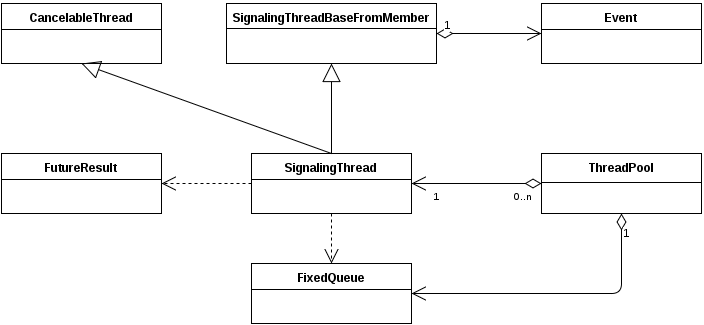
\includegraphics[width=1.0\textwidth]{img/class_diag.png}
  \caption{Дијаграм класа}
  \label{fig:klasa_dij}
\end{figure}

\section{Интеграција модула са системом LAV}

Паралелизација је имплементирана у контексту анализе наредби и функција модула који се верификује. 

\subsection{Паралелна анализа наредби}

Класа \texttt{LBlock} система \textit{LAV} служи за рад са блоковима кода. Њена функција \texttt{CalculateConditions} конструише формуле које представљају услове исправности блока и позивају \textit{SMT} решавач за сваку формулу. Модул за паралелизацију омогућава да се ови позиви решавача извршавају паралелно.

 За сваку формулу услова исправности, унутар функције \texttt{CalculateConditions} конструише се функција која позива \textit{SMT} решавач. Функција као резултат враћа индикатор да ли је услов исправности испуњен или не. Направљене функције се смештају у ред \texttt{FixedQueue} и прослеђују инстанци класе \texttt{ThreadPool} (складиште нити). Складиште нити прави радне нити и покреће их. Свака нит извршава једну по једну функцију, узимајући их из реда и обавештава складиште нити о резултату извршавања. Уколико се наиђе на услов исправности који није задовољен, нема потребе испитивати остале услове јер се тада блок сматра неисправним. У контексту имплементације то значи да уколико нека функција врати индикатор да услов исправности није испуњен, нити могу престати са радом јер се задат блок означава као неисправан. Ако је приликом покретања система \textit{LAV} (била) задата опција \texttt{-find-first-flawed} и ако нека функција врати индикатор да услов исправности није испуњен, онда све остале нити могу да престану са радом јер се задат блок означава као неисправан. Ако та опција није присутна, онда се испитују сви услови исправности. Када све функције из реда заврше тако да су сви услови били задовољени, блок се сматра исправним и тако бива означен. 
 
 На слици \ref{fig:sekv_dij}  је приказан један могући сценарио. На почетку се врши конструкција и иницијализација свих потребних објеката. Складиште нити конструише три радне нити које узимају задатке са реда. Нит \texttt{SignalingThread1} прва узима задатак из реда, а након ње и \texttt{SignalingThread2} и обе почињу да их извршавају. Нит \texttt{SignalingThread1} прва завршава успешно, пре него што је нит \texttt{SignalingThread3} узела задатак из реда. Након тога нити  \texttt{SignalingThread1} и  \texttt{SignalingThread3} покушају да узму следећи задатак. Имајући у виду то да један ред задатака деле све нити, овај процес узимања задатака ће се извршити секвенцијално (користећи погодне функције из библиотеке  \texttt{<atomic>}) тако да нит \texttt{SignalingThread1} прва добија задатак из реда. Како нит  \texttt{SignalingThread1} наилази на услов исправности који није испуњен, шаље сигнал складишту нити након чега остале нити бивају заустављене и систем \textit{LAV} бива обавештен о неисправном резултату. Можемо приметити да је редослед акција прављења нити, скидање задатака из реда и брзина извршавања задатака у овом примеру конкретизован. Наравно, у општем случају тај редослед је произвољан и зависи од много фактора као што су специфичности оперативног система, сложеност задатака, број задатака у реду, и слично.  


\begin{figure}[!ht]
  \centering
  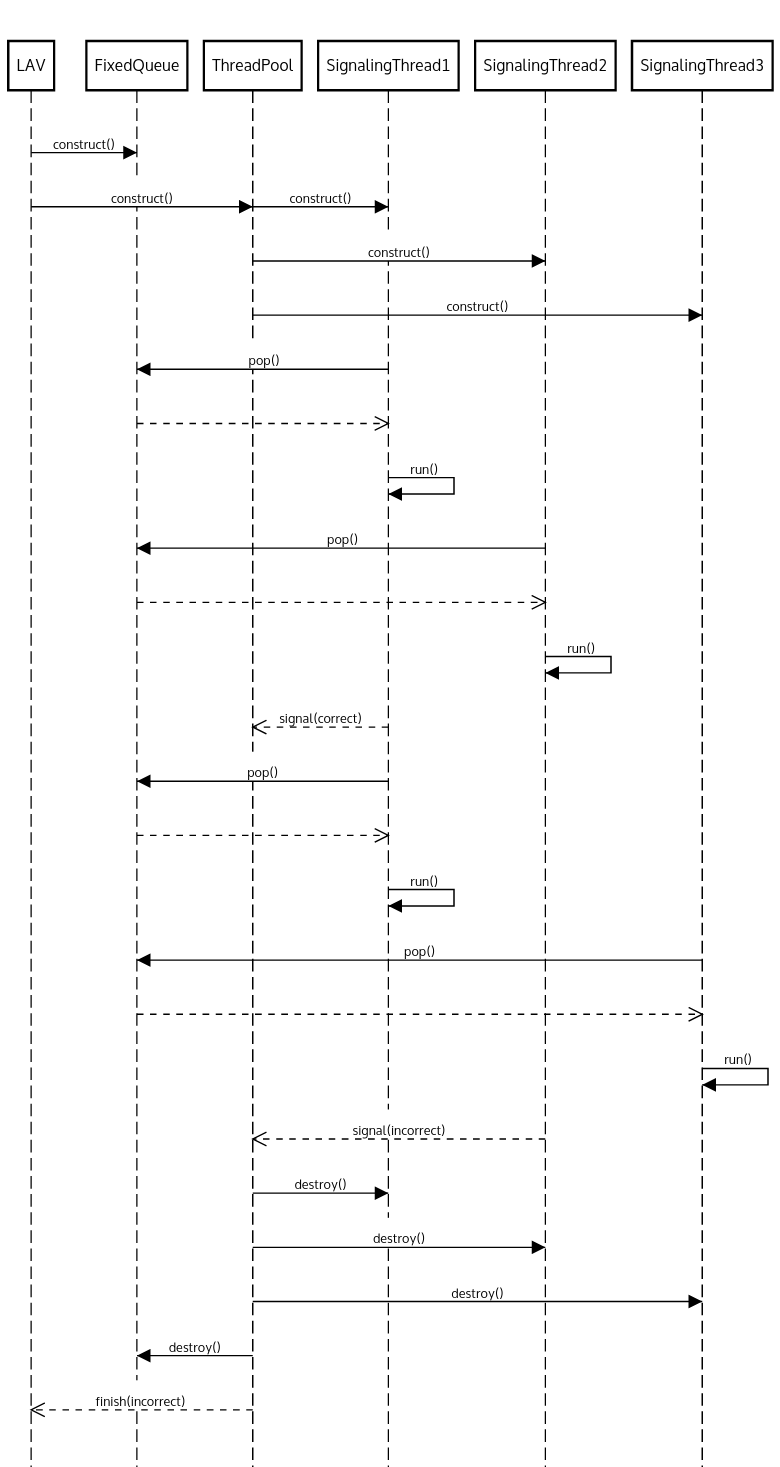
\includegraphics[width=0.8\textwidth]{img/seq_diag.png}
  \caption{Дијаграм тока извршавања програма са више нити}
  \label{fig:sekv_dij}
\end{figure}

\subsection{Паралелна анализа функција}

Анализа функција је имплементирана уз употребу истих механизама уз мале додатке због различитости проблема.   
 Класа \texttt{LModule} је одговорна за анализу функција једног модула. Функције могу зависити једне од других због чега је потребно чувати информације о резултату верификације сваке функције појединачно. Верификација модула почиње позивом методе \texttt{Run} класе \texttt{LModule} у оквиру кога се конструишу нити које анализирају функције тог модула. Класи \texttt{LModule} је додат низ објеката \texttt{FutureResult} за сваку од функција тог модула. Класа \texttt{FutureResult} представља структуру података унутар које се чува податак о завршетку верификације неке функције. Ова класа садржи објекат класе \texttt{std::promise}  који чува вредност (информацију о завршетку верификације) и објекат \texttt{std::future} помоћу кога нити приступају тој вредности. Свака нит има дељени показивач на низ објеката \texttt{FutureResult} тако да у сваком тренутку може погледати резултат верификације неке друге функције. Уколико се верификација тражене функције није завршила, тренутна нит ће сачекати да се она заврши позивом функције \texttt{wait} над објектом \texttt{std::future} за ту функцију. Када се верификација тражене функције заврши, резултат ће се уписати у њен објекат \texttt{std::promise} и функција \texttt{wait} ће завршити са чекањем. . Уколико је задата опција \texttt{-find-first-flawed} приликом наиласка на неисправну функцију онда се програм означава као неисправан, а остале нити се отказују, чиме се верификација завршава. Иначе остале нити настављају са радом и тек након њиховог завршетка се верификација завршава.

\chapter{Експериментални резултати}

У наставку текста ће бити приказани резултати поређења модификованог система \textit{LAV} са алатом \textit{CBMC}. Корпуси на коме су тестиране алатке, добијени резултати и све потребне скрипте за генерисање корпуса, покретање и чување резултата су јавно доступне и могу се пронаћи на адреси \url{http://argo.matf.bg.ac.rs/?content=lav}.


  \section{Архитектура рачунара}
  
  С обзиром на то да се рад заснива на паралелној импмементацији, експерименти су покретани на кластер рачунару са четрдесет и осам процесорских језгара, \textit{94GB} радне меморије и оперативним системом \textit{Ubuntu} 16.04. Максимално време извршавања програма је постављено на 400 секунди. Време је мерено системским програмом \texttt{time}.
  
  \section{Опис корпуса}
  
  Експерименти су покретани на два корпуса, први демонстрира побољшање услед паралелне верификације блокова, а други демонстрира побољшање услед паралелне верификације функција програма.
  \subsection{Први корпус}
  
 Овај корпуса има за циљ да провери како се понаша паралелизације наредби услед великог броја сложених наредби у једном блоку. Корпус садржи двадесет програма писаних у програмском језику \textit{C}. Сви програми у корпусу су конструисани на основу наведеног примера повећавајући број наредби. Програми су преведени у \textit{32b} и \textit{64b} режиму како би се испитало да ли постоји значајна разлика у резултатима. Експерименти су показали да велика разлика не постоји, и због тога су се програми другог корпуса преводили само у \textit{32b} режим. 

  
\begin{lstlisting}[basicstyle=\fontsize{12}{4}\selectfont,language=C,frame=single,caption=Пример програма,label=primer1]

int m(int a, int b, int c, int d) {

	// --- I skup ---
	// naredbe koje simuliraju slozena izracunavanja
	a = (b<<3)*((c>>2)/3);
	b = (a<<3)*((c>>2)/3);
	c = (b<<3)*((a>>2)/3);

	// --- II skup --- 
	// naredbe koje mogu dovesti do deljenja nulom
	a = b/c + b/a + c/(++b);
	b = a/d;
	
	return b;
}
\end{lstlisting}
 Програми су генерисани копирањем наредби из првог скупа. Број копирања за сваки генерисани програм расте, и припада интервалу $[1,60]$. Понављање ових наредби симулира комплексна израчунавања која блок потенцијално може да садржи. За наредбе другог скупа је потребно утврдити да ли могу да доведу до дељења нулом. На пример, провера да ли су вредности израза \texttt{a}, \texttt{++b} и \texttt{c} различите од нуле укључује комплексне формуле настале симболичким извршавањем наредби првог скупа, док је провера да ли је вредност променљиве \texttt{d} различита од нуле једноставна.    


\subsection{Други корпус}

Наредни корпус се састоји од програма који садрже одређен број функција како би се демонстрирала верификација мало сложенијих програма. Корпус је подељен у две категорије од којих свака има две верзије и садржи укупно 2000 програма писаних у програмском језику \textit{C}. Програми овог корпуса не садрже наредбе неисправног дељења како би процес верификације обухватио пролазак кроз све путање програма (што је захтевније него у случају када се проналажењем грешке прекида извршавање).

\paragraph{Прва категорија} садржи програме са различитим бројем функција (од једне до педесет функција). Свака функција се састоји од одређеног број наредби које симулирају комплексна извршавања. Повећањем броја наредби отежава се провера коректности функција као и самог програма. Испитивање коректности потенцијално проблематичне наредбе дељења у првој верзији ове категорије не зависи од резултата претходних израчунавања, док у другој верзији зависи од резултата претходних израчунавања. Ово својство чини услове испитивања исправности лакшим у односу на програме друге верзије. Главна функција \texttt{main} позива све постојеће функције, због чега је за испитивање исправности програма потребно испитати исправност свих функција. Примери програма прве и друге верзије ове категорије се могу видети на сликама \ref{primer_nivo_1} и \ref{primer_nivo_1t}.

\paragraph{Друга категорија} се састоји од програма са различитим бројем функција које садрже позиве других функција. Повећањем дубине позива функција значајно се компликује испитивање коректности програма. Свака функција, као и у првој категорији, садржи наредбе које симулирају комплексна израчунавања и потенцијално проблематичне наредбе дељења. Такође, прва и друга, односно лакша и тежа, верзија ове категорије се разликују по сложености проблематичних наредби. Примери програма прве и друге верзије ове категорије се могу видети на сликама \ref{primer_nivo_2} и \ref{primer_nivo_2t}.
 
\begin{lstlisting}[basicstyle=\fontsize{12}{4}\selectfont,language=C,frame=single,caption=Пример програма прве категорије (прва верзија),label=primer_nivo_1]

int f1(int a, int b, int c) {

 // naredbe koje simuliraju slozena izracunavanja
 a = (b<<1)*((a>>1)/3);
 b = (a<<1)*((b>>1)/3);
  
 if(c!=0)
 // naredba deljenja za koju je potrebno utvrditi ispravnost
   return a/c;
   
 return a+b;
}

int main() {
 int a, b, c, r = 0;
 
 scanf("%d%d%d", &a, &b, &c);
 
 r += f1(a,b,c);
 
 return r;
}

\end{lstlisting}

\begin{lstlisting}[basicstyle=\fontsize{12}{4}\selectfont,language=C,frame=single,caption=Пример програма прве категорије (друга верзија),label=primer_nivo_1t]

int f1(int a, int b) {

 // naredbe koje simuliraju slozena izracunavanja
 a = (b<<1)*((a>>1)/3);
 b = (a<<1)*((b>>1)/3);
 
 if(b!=0)
 // naredba deljenja za koju je potrebno utvrditi ispravnost
   return a/b;
 
 return a+b;
}

int main() {
 int a, b, r = 0;
 
 scanf("%d%d", &a, &b);
 
 r += f1(a,b);

 return r;
}

\end{lstlisting}

\begin{lstlisting}[basicstyle=\fontsize{12}{4}\selectfont,language=C,frame=single,caption=Пример програма друге категорије (прва верзија),label=primer_nivo_2]

int _f1(int a, int b, int c) {

 // naredbe koje simuliraju slozena izracunavanja
 a = (b<<1)*((a>>1)/3);
 b = (a<<1)*((b>>1)/3);

 if(c!=0)
 // naredba deljenja za koju je potrebno utvrditi ispravnost
   return a/c;

 return a+b+c;
}

int f1(int a, int b, int c) {

 // naredbe koje simuliraju slozena izracunavanja
 a = (b<<1)*((a>>1)/3);
 b = (a<<1)*((b>>1)/3);

 if(c!=0)
 // naredba deljenja za koju je potrebno utvrditi ispravnost
 // i poziv druge funkcije 
   return a/c + _f1(a,b,c);

 return a+b+c;
}

int main() {

 int a, b, c, r = 0;

 scanf("%d%d%d", &a, &b, &c);

 r += f1(a,b,c);

 return r;
}


\end{lstlisting}



\begin{lstlisting}[basicstyle=\fontsize{12}{4}\selectfont,language=C,frame=single,caption=Пример програма друге категорије (друга верзија),label=primer_nivo_2t]
#include <stdio.h>

int _f1(int a, int b, int c) {

 // naredbe koje simuliraju slozena izracunavanja 
 a = (b<<1)*((a>>1)/3);
 b = (a<<1)*((b>>1)/3);
 
 if(b!=0)
 // naredba deljenja za koju je potrebno utvrditi ispravnost
   return a/b;
   
 return a+b+c;
}

int f1(int a, int b, int c) {

 // naredbe koje simuliraju slozena izracunavanja 
 a = (b<<1)*((a>>1)/3);
 b = (a<<1)*((b>>1)/3);
 
 if(b!=0)
 // naredba deljenja za koju je potrebno utvrditi ispravnost
 // i poziv druge funkcije 
   return a/b + _f1(a,b,c);
   
 return a+b+c;
}

int main() {
 int a, b, c, r = 0;
 
 scanf("%d%d%d", &a, &b, &c);
 
 r += f1(a,b,c);
 
 return r;
}


\end{lstlisting}



\subsection{Начини покретања}
%
%Приликом покретања алата LAV и CBMC над инстанцама програма првог и другог корпуса, коришћене су различите заставице и параметри како би се што боље демонстрирао рад алата и њихова ефикасност. У наставку ће бити описани начини покретања оба алата за програме из оба корпуса.
%
%\subsubsection{Први корпус}

Приликом покретања алата над инстанцама програма из овог корпуса алат \textit{LAV} је покретан са опцијом заустављања приликом наиласка на прву неисправну наредбу, решавач који је коришћен је \textit{Z3}. Број нити које користи \textit{LAV} није експлицитно задат\footnote{То је број потребних нити односно број који је добијен као препорука оперативног система (и не мора представљати број физичких језгара на рачунару) уколико је потребно више нити него што систем дозвољава.}. Алат \textit{CBMC} је покретан са параметром који испитује проблем дељења нулом. Име функције чију исправност је потребно испитати се експлицитно задаје заставицама \texttt{-starting-function=m} и \texttt{--function m} приликом покретања оба алата над програмима првог корпуса. Верификација инстанци другог корпуса подразумева испитивање исправности свих функција у програму и због тога није потребно задавање поменутих заставица јер је подразумевана почетна функција \texttt{main}.
\\ \\
Пример покретања \textit{LAV}-а:
\\ \\
\texttt{./LAV 25\_lines.o -solver=Z3-BV-ARR-EUF -find-first-flawed -enable-parallel -starting-function=m}
\\ \\
Пример покретања \textit{CBMC}-а:
\\ \\
\texttt{./CBMC --div-by-zero-check --32 --function m 25\_lines.c}

%\subsubsection{Други корпус}

  
 \section{Анализа резултата}
	У наставку ће бити изложена анализа резултата који су добијени покретањем алатки \textit{LAV} и \textit{CBMC} над програмима из коришћених корпуса. 	
	
  Добијени резултати приликом верификације програма из првог корпуса се налазе у табели \ref{eksp_blok}, измерена времена су приказана у секундама. 
  
  Резултати показују да је време потребно алату \textit{CBMC} за верификацију значајно веће од времена које је потребно алату \textit{LAV} уз коришћење имплементиране паралелизације на нивоу блока. Са повећањем броја наредби, повећавају се формуле које описују програм и чију задовољивост је потребно испитати, због чега се укупно време потребно за верификацију драстично увећава. Приметимо да је време потребно за верификацију програма који садржи двадесет и шест наредби користећи алат \textit{CBMC} више него двоструко веће од времена које је потребно за верификацију програма од двадесет и пет наредби, док је разлика тих времена при употреби алата \textit{LAV} мала. Овакви резултати показују да паралелним испитивањем исправности наредби програма можемо драстично смањити укупно време које је потребно за верификацију и на тај начин унапредити постојеће алатке.
  
\begin{table}
  \begin{tabularx}{1\textwidth}{|>{\setlength\hsize{1\hsize}\centering}X|>{\setlength\hsize{1\hsize}\centering}X|>{\setlength\hsize{1\hsize}\centering}X|>{\setlength\hsize{1\hsize}\centering}X|X|}
  \hline
  	\multirow{2}{*}{број наредби} & \multicolumn{2}{ c }{32b} &\multicolumn{2}{ | c | }{64b} 
	\\
	\cline{2-5}
	& LAV & CBMC & LAV & CBMC \\	
	\cline{1-5}
	12 & 0.08 & 0.72       & 0.07 & 0.82   \\	
	\cline{1-5}
	13 & 0.23 & 0.75       & 0.25 & 0.72   \\	
	\cline{1-5}
	14 & 0.38 & 0.93       & 0.08 & 0.93   \\	
	\cline{1-5}
	15 & 0.08 & 1.21       & 0.08 & 1.10   \\	
	\cline{1-5}
	16 & 0.27 & 1.42       & 0.09 & 1.46   \\	
	\cline{1-5}
	17 & 0.08 & 2.16       & 0.10 & 2.15   \\	
	\cline{1-5}
	18 & 0.10 & 3.08       & 0.23 & 3.05   \\	
	\cline{1-5}
	19 & 0.26 & 4.12       & 0.09 & 4.15   \\	
	\cline{1-5}
	20 & 0.11 & 7.80       & 0.21 & 7.93   \\	
	\cline{1-5}
	21 & 0.11 & 11.73      & 0.23 & 12.09  \\	
	\cline{1-5}
	22 & 0.22 & 16.50       & 0.23 & 17.28  \\	
	\cline{1-5}
	23 & 0.09 & 33.91      & 0.10 & 34.78  \\	
	\cline{1-5}
	24 & 0.11 & 52.50      & 0.10 & 53.46  \\	
	\cline{1-5}
	25 & 0.12 & 75.32      & 0.09 & 74.72  \\	
	\cline{1-5}
	26 & 0.11 & 157.01     & 0.10 & 154.87  \\	
	\cline{1-5}
	27 & 0.13 & 246.89     & 0.12 & 253.92  \\	
	\cline{1-5}
	28 & 0.12 & $\nearrow$ & 0.12 & $\nearrow$ \\	
	\cline{1-5}
	29 & 0.12 & $\nearrow$ & 0.13 & $\nearrow$ \\	
	\cline{1-5}
	30 & 0.14 & $\nearrow$ & 0.13 & $\nearrow$ \\	
	\cline{1-5}
	60 & 0.18 & $\nearrow$ & 0.20 & $\nearrow$ \\	
   \cline{1-5}
  \end{tabularx}

\caption[]{Експериментални резултати алатки LAV и CBMC на првом корпусу {\label{eksp_blok}}}
\end{table}


  Резултати верификације програма из другог корпуса су приказани на графицима \ref{fig:nivo_1}, \ref{fig:nivo_1t}, \ref{fig:nivo_2} и \ref{fig:nivo_2t}. Алатке су покретане са ограничењем времена на 400 секунди. Ради прегледности графика нису приказани сви резултати, већ су одабрани они резултати који показују одговарајући тренд раста.
  
  На графицима \ref{fig:nivo_1} и \ref{fig:nivo_2} се може видети да време потребно алату \textit{CBMC} значајно расте услед повећања броја наредби у функцијама програма.  Такође можемо приметити да пораст времена зависи и од броја функција у програму. Алат \textit{CBMC} достиже временско ограничење од 400 секунди већ на инстанци програма која садржи десет функција са шест наредби и још једним нивоом позива (тамна испрекидана линија на графику \ref{fig:nivo_2}). 
  
  Време које је потребно алату \textit{LAV} не расте великом брзином уколико повећавамо број наредби односно функција. што је резултат паралелног испитивања задовољивости \textit{SMT} формула. Како проблематичне наредбе програма овог корпуса не зависе од резултата претходних сложених наредби, могуће је скоро па потпуно паралелизовати испитивање њихове коректности, и тиме умањити укупно потребно време. 
  
  Ако посматрамо однос времена које је утрошено коришћењем алата \textit{LAV} и алата \textit{CBMC}, можемо закључити да је паралелизација имплементирана унутар алата \textit{LAV} значајно смањила (у неким случајевима за ред величина већи од $ 10^{2} $, љубичасте линије на графицима \ref{fig:nivo_1} и \ref{fig:nivo_2}) потребно време за верификацију програма из овог корпуса.
  
  На графицима \ref{fig:nivo_1t} и \ref{fig:nivo_2t} можемо да видимо измерена времена над инстанцама програма прве и друге категорије чија коректност се теже испитује. Ови програми, као што је описано у претходном поглављу, садрже проблематичне наредбе које зависе од резултата израчунавања претходних сложених наредби. Ово својство програма чини формуле чија се исправност испитује тежим, што резултује порастом времена потребног за верификацију. Али, и поред описаног ограничења, паралелизована верзија алата \textit{LAV} потроши мању количину времена приликом верификације сложенијих програма у поређењу са алатом \textit{CBMC}. Време потребно \textit{LAV}-у за верификацију једноставнијих програма који садрже мањи број наредби је, у неким ситуацијама, веће од времена које је потребно алату \textit{CBMC}. Ово показује да се паралелизација не исплати у свим ситуацијама јер конструисање контекста, прављење, покретање и синхронизација нити кошта односно троши одређено време.  
  
\newpage
\begin{figure}[!ht]
  \centering
  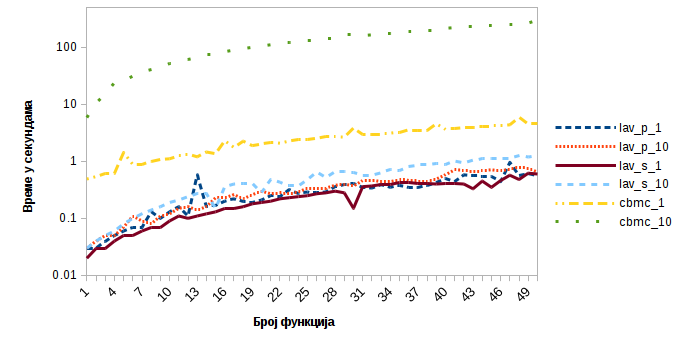
\includegraphics[scale=0.8]{img/nivo1_master.png}
  \caption{Прва категорија, лакша верзија, линија обележена \texttt{lav\_p\_1} односно \texttt{lav\_p\_10} приказује времена потребна алату \textit{LAV} да паралелни приступом верификује програм са једним односно десет блокова наредби, аналогно је за секвенцијални приступ као и за алат \textit{CBMC}}
  \label{fig:nivo_1}
\end{figure}

\begin{figure}[!ht]
  \centering
  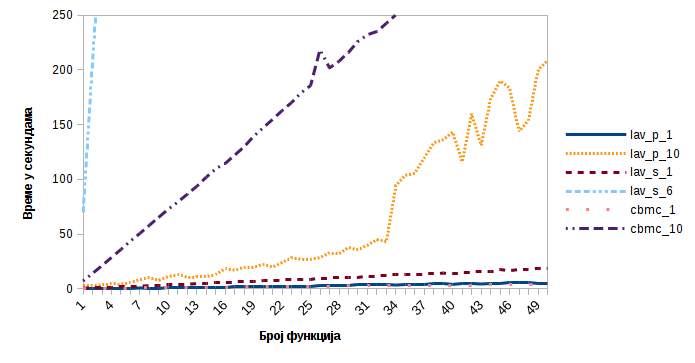
\includegraphics[scale=0.8]{img/nivo1T_master.png}
  \caption{Прва категорија, тежа верзија, линија обележена \texttt{lav\_p\_1} односно \texttt{lav\_p\_10} приказује времена потребна алату \textit{LAV} да паралелни приступом верификује програм са једним односно десет блокова наредби, аналогно је за секвенцијални приступ као и за алат \textit{CBMC}}
  \label{fig:nivo_1t}
\end{figure}

\begin{figure}[!ht]
  \centering
  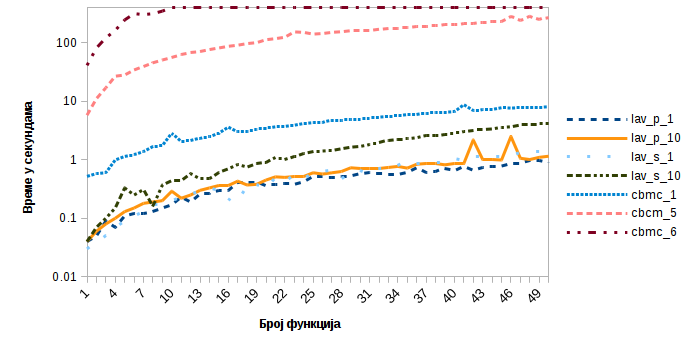
\includegraphics[scale=0.8]{img/nivo2_master.png}
  \caption{Друга категорија, лакша верзија, линија обележена \texttt{lav\_p\_1} односно \texttt{lav\_p\_10} приказује времена потребна алату \textit{LAV} да паралелни приступом верификује програм са једним односно десет блокова наредби, аналогно је за секвенцијални приступ као и за алат \textit{CBMC}}
  \label{fig:nivo_2}
\end{figure}

\begin{figure}[!ht]
  \centering
  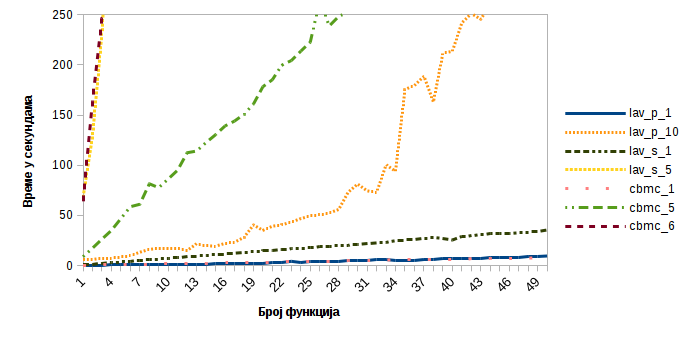
\includegraphics[scale=0.8]{img/nivo2T_master.png}
  \caption{Друга категорија, тежа везија, линија обележена \texttt{lav\_p\_1} односно \texttt{lav\_p\_10} приказује времена потребна алату \textit{LAV} да паралелни приступом верификује програм са једним односно десет блокова наредби, аналогно је за секвенцијални приступ као и за алат \textit{CBMC}}
  \label{fig:nivo_2t}
\end{figure}


\chapter{Закључак} 

У овом раду разматран је проблем захтевности процеса верификације програма. Имплементирана је надоградња систему за верификацију \textit{LAV} која паралелизује испитивање исправности софтвера на два нивоа, паралелном верификацијом блокова кода и паралелном верификацијом функција програма.

Унапређен алат \textit{LAV} је тестиран на програмима из два корпуса. Инстанце програма првог корпуса су састављене са циљем да демонстрирају сложеност испитивања исправности блокова кода који садрже наредбе са комплексним израчунавањима. Програми другог корпуса садрже променљив број функција са различитим бројем наредби и дубином позива функција како би се показала временска захтевност верификације програма који садрже више од једне функције, што је најчешћи случај у данашњим софтверским решењима.

Изложени су експериментални резултати као и упоредна анализа алата \textit{LAV} са сродним алатом \textit{CBMC}. Резултати показују да за велике и комплексне програме предложено унапређење алата \textit{LAV} значајно скраћује време потребно за утврђивање исправности програма. Приликом верификације једноставнијих програма дешава се да процес паралелизације захтева више времена него сама верификација, тако да је у тим случајевима није погодно користити.

Будућа истраживања на тему унапређења алата за верификацију би могла обухватити примене различитих метода машинског учења приликом одабира подскупа \textit{SMT} формула чија задовољивост ће прва бити испитана. Још један смер побољшања може бити смањивање броја \textit{SMT} формула као и њихово појединостављивање како би се редуковало време потребно за испитивање задовољивости.


\literatura
% ==============================================================================
% Završni deo teze i prilozi
\backmatter
\end{document}
